\documentclass[twocolumn]{article}

\title{Intersection of lines}
\author{Paul Maynard}

\usepackage{amsmath, amsthm}
\usepackage{hyperref}
\usepackage{tikz}
\usetikzlibrary{patterns}
% \usepackage[outline]{contour}



\newtheorem{theorem}{Theorem}

\begin{document}
\maketitle

\begin{abstract}
This document outlines a method for determining how many slices two lines divide a circle into.
\end{abstract}

\section{Setup}
Consider two lines each defined by two points on a circle,
$P_1$ and $P_2$, $Q_1$ and $Q_2$, as in Figure~\ref{fig:2lines}. 

\vspace{1pc}

\begin{figure}[h]
\centering
\caption{Two lines}
\label{fig:2lines}
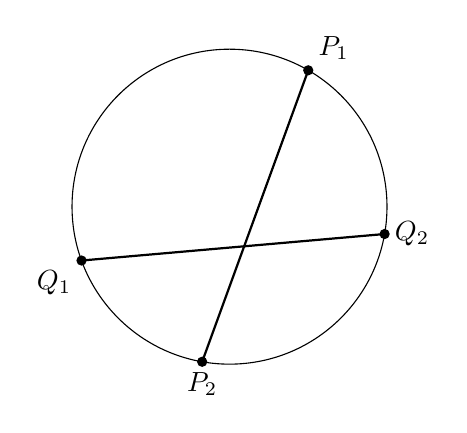
\begin{tikzpicture}[scale=2,>=latex]
    % \draw [<->,gray] (1.2,0) -- (0,0) -- (0,1.2);
    \draw (0,0) circle [radius=1];
    \draw [fill,thick] (60:1) circle [radius=.025]
                        node [above right] {$P_1$}
                  -- (-100:1) circle [radius=.025]
                              node [below] {$P_2$};
    
    \draw [fill,thick] (-10:1) circle [radius=.025]
                        node [right] {$Q_2$}
                  -- (-160:1) circle [radius=.025]
                              node [below left] {$Q_1$};
\end{tikzpicture}
\end{figure}

These lines can obviously intersect or not. If they intersect, then the circle is cut into four regions.
If they don't then it is cut into three. This intersection can be checked 
without reference to the lines, but by simply looking at the angles of the points.

If $P_1$ and $P_2$ are ``next to'' each other, that is, there i no point between them, then they do not intersect any point.
On the other hand, if there is a point between them, but not that points counterpart, then that point's line will intersect it.

\begin{figure}[h]
\centering
\caption{Intersecting vs.\ Non-intersecting lines}
\label{fig:intersect}
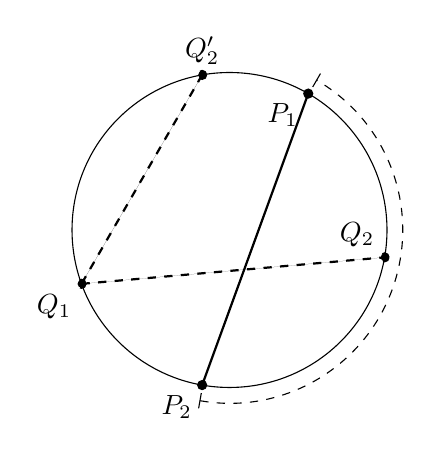
\begin{tikzpicture}[scale=2,>=latex]
    % \draw [<->,gray] (1.2,0) -- (0,0) -- (0,1.2);
    \draw (0,0) circle [radius=1];
    \draw [fill,thick] (60:1) circle [radius=.025]
                        node [below left] {$P_1$}
                  -- (-100:1) circle [radius=.025]
                              node [below left] {$P_2$};
    
    \draw [fill,thick,dashed] (100:1) circle [radius=.025]
                                      node [above] {$Q_2^{\prime}$}
                          -- (-160:1) circle [radius=.025]
                                      node [below left] {$Q_1$}       
                          -- (-10:1) circle [radius=.025]
                                     node [above left] {$Q_2$};
    \draw [|-|,thin,dashed] (-100:1.1) arc (-100:60:1.1);
\end{tikzpicture}
\end{figure}

We can see in Figure~\ref{fig:intersect} that the line $\overline{Q_1 Q_2}$ intersects $\overline{P_1 P_2}$,
while $\overline{Q_1 Q_2^{\prime}}$ does not. In fact, any placement of $Q_2$ within the dashed interval
will result in an intersection, while any outside will not. This, in order to check fot intersection, it is sufficient to check the sequence of angles.

\section{Probability}

\begin{figure}[h]
    \centering
    \caption{Angle Configuration}
    \label{fig:config}
    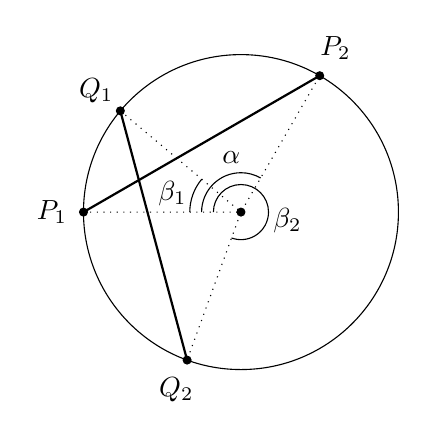
\begin{tikzpicture}[scale=2,>=latex]
        \draw (0,0) circle [radius=1];
        \draw [fill] (0,0) circle [radius=.025];
    
        \draw [thick] (180:1) -- (60:1);
        \draw [dotted] (180:1) -- (0,0) -- (60:1);
        \draw (180:.25) arc (180:60:.25);
        \draw (100:.35) node {$\alpha$};
        \draw [fill] (180:1) circle [radius=.025] ++ (180:.2) node {$P_1$};
        \draw [fill] (60:1) circle [radius=.025] ++ (60:.2) node {$P_2$};
    
        \draw [dotted] (140:1) -- (0,0) -- (-110:1);
        \draw [thick] (140:1) -- (-110:1);
        \draw (180:.325) arc (180:140:.325);
        \draw (165:.45) node {$\beta_1$};
        \draw (180:.175) arc (180:-110:.175);
        \draw (-10:.3) node {$\beta_2$};
        \draw [fill] (140:1) circle [radius=.025] ++ (140:.2) node {$Q_1$};
        \draw [fill] (-110:1) circle [radius=.025] ++ (-110:.2) node {$Q_2$};
    \end{tikzpicture}
\end{figure}

To calculate the probability of different amounts of spaces, consider the possible variables.
Since the configuration is preserved under rotation, it is sufficient to consider the
angles of the points from $P_1$. In Figure~\ref{fig:config}, the angle between 
$P_1$ and $P_2$ is $\alpha$, and $\beta_1$ and $\beta_2$ are the angles of $Q_1$
and $Q_2$ from $P_1$. There are two possible types of configurations of these lines:

\begin{enumerate}
    \item $\beta_1, \beta_2 \le \alpha$ or $\beta_1, \beta_2 \ge \alpha$.
          In this case, there will be no intersection, so they divide the circle into three regions
    \item $\beta_1 < \alpha < \beta_2$ or $\beta_1 > \alpha > \beta_2$.
          In this case, the lines intersect, so there are four regions.
\end{enumerate}

\begin{figure}[h]
    \centering
    \caption{Configuration space}
    \label{fig:space}
    \begin{tikzpicture}[scale=2,>=latex]
        % \fill [pattern=vertical lines] (0,1.3) rectangle (1.3,2);
        \draw [thin] (-.1,2) -- (2,2) -- (2,-.1) node [below] {$2\pi$};
        \draw [<->,thick] (0,2.2) node [above] {$\beta_2$} -- (0,0)
            -- (2.2,0) node [right] {$\beta_1$};
        \draw [dashed] (2.1,1.3) -- (-.1,1.3);
        \draw [dashed] (1.3,2.1) -- (1.3,-.1) node [below] {$\alpha$};

        \node at (.65,.65) {3};
        \node at (1.65,1.65) {3};
        \node at (.65,1.65) {4};
        \node at (1.65,.65) {4};
    \end{tikzpicture}
\end{figure}


\end{document}